\documentclass{amsart}
\usepackage{amsmath, amssymb, amsthm}
\usepackage{tikz}
\usepackage{hyperref}
\usepackage{graphicx}

\newtheorem{theorem}{Theorem}[section]
\newtheorem{corollary}[theorem]{Corollary}

\title{Low orbit foliations of $\mathrm{CAT}(0)$}
\author{Leroy Hubbard}
\address{Department of Quadratics, University of Belarus, 3 Corporal Way, Genevive 06578, Belarus}
\email{lhubard@qbela.edu}

\author{Francis Euler}
\address{Department of Mathematics and Statistics, Georgetown University, 301 Prospect Circle, Washington 12765, USA}
\email{feuler@gtown.edu}

\thanks{L.\ H.\ was supported by NSF grant No.\ 314159357. F.\ E.\ thanks the Department of Linguistics for the valuable conversations.}


\newwrite\markfile
\immediate\openout\markfile=boxpositions_source0.txt

\newcommand{\markbox}[2]{%
  \setbox0=\hbox{#2}%
  \immediate\write\markfile{#1:whd{}:\the\value{page}:\the\wd0:\the\ht0:\the\dp0}%
  \pdfsavepos
  \write\markfile{#1:start:\the\value{page}:\the\pdflastxpos:\the\pdflastypos}%
  #2% 
  \pdfsavepos
  \write\markfile{#1:end{}:\the\value{page}:\the\pdflastxpos:\the\pdflastypos}%
}


\renewcommand{\eqref}[1]{(\ref{#1})}
\begin{document}
\begin{abstract}
We set $\mathcal{G} = \sim\frac{\lambda^2}{[H : K]}$ and investigate the orbits of 
$\mathfrak{I} = \frac{\mathrm{CAT}(0)}{\mathcal{G}^{\lambda k}}$ 
provided $\lambda \in [1-\varphi, 1+\varphi]$, where $\varphi$ is the golden ratio. 
Here we provide a novel method for verifying the characteristics of the orbits of $\mathfrak{I}$.
\end{abstract}

\maketitle


\section{Introduction}

Ever \markbox{0}{since} 1689 \markbox{1}{with} Fermat's \markbox{2}{treatise} \markbox{3}{on} \markbox{4}{prime} \markbox{5}{enumeration} \cite{fermat89}, 
attempts \markbox{6}{at} \markbox{7}{understanding} \markbox{m8}{$\frac{\mathrm{CAT}(0)}{\mathcal{G}^{\lambda k}}$} \markbox{9}{have} \markbox{10}{been} \markbox{11}{underway} \markbox{12}{but} \markbox{13}{mostly} unsuccessful. 
Our \markbox{14}{main} \markbox{15}{objective} \markbox{16}{is} \markbox{17}{to} \markbox{18}{describe} \markbox{19}{the} low-orbit \markbox{20}{foliations} \markbox{21}{induced} \markbox{22}{by} \markbox{m23}{$\mathfrak{I}$} \markbox{24}{on} 
the pseudo-Euclidean \markbox{25}{completion} \markbox{26}{of} \markbox{27}{a} \markbox{m28}{$\mathrm{CAT}(0)$} complex. 
This \markbox{29}{perspective} \markbox{30}{arose} \markbox{31}{from} \markbox{32}{the} \markbox{33}{need} \markbox{34}{to} \markbox{35}{understand} \markbox{36}{the} \markbox{37}{failure} \markbox{38}{of} \markbox{39}{the} ``Flat \markbox{40}{Orbit} Conjecture'' \markbox{41}{in} \markbox{42}{higher} \markbox{43}{curvature} regimes\footnote{
Originally conjectured by P.\ Alexandrov, the Flat Orbit Conjecture proposed that all $\lambda$-periodic orbits of a $\mathrm{CAT}(0)$ space are isometric to Euclidean circles. 
This is now known to be false in dimensions $\geq 3$ due to \cite{hubard23}.}.

\section{Background and Preliminaries}



Let \markbox{m44}{$(X,d)$} \markbox{45}{be} \markbox{46}{a} \markbox{m47}{$\mathrm{CAT}(0)$} \markbox{48}{space} \markbox{49}{in} \markbox{50}{the} \markbox{51}{sense} \markbox{52}{of} Gromov.  
For \markbox{53}{a} \markbox{54}{fixed} \markbox{m55}{$\lambda > 0$}, \markbox{56}{define} \markbox{57}{the} \emph{low orbit foliation} \markbox{m58}{$\mathcal{F}_\lambda(X)$} as
\begin{equation}\label{eq:foliation}
    \mathcal{F}_\lambda(X) = \{\,x \in X \mid \Delta(x, \lambda) = \text{const.}\,\},
\end{equation}
where \markbox{m59}{$\Delta(x, \lambda) = d(x, \lambda x)$} \markbox{60}{denotes} \markbox{61}{the} \markbox{62}{displacement} \markbox{63}{function} \markbox{64}{under} \markbox{m65}{$\lambda$}-scaling.  
This \markbox{66}{function} \markbox{67}{is} \markbox{68}{trivially} \markbox{69}{constant} \markbox{70}{when} \markbox{m71}{$X$} \markbox{72}{is} Euclidean, \markbox{73}{but} \markbox{74}{varies} \markbox{75}{dramatically} \markbox{76}{in} non-flat \markbox{m77}{$\mathrm{CAT}(0)$} manifolds.

\subsection{A remark on $\mathcal{G}$-stabilizers}
We \markbox{78}{shall} \markbox{79}{repeatedly} \markbox{80}{use} \markbox{81}{the} \markbox{82}{stabilizer} group
\[
    \mathrm{Stab}_{\mathcal{G}}(x) = \{ g \in \mathcal{G} \mid g \cdot x = x \},
\]
whose \markbox{83}{index} \markbox{m84}{$[\mathcal{G} : \mathrm{Stab}_{\mathcal{G}}(x)]$} \markbox{85}{determines} \markbox{86}{the} \emph{orbit density} \markbox{87}{at} \markbox{m88}{$x$}.  
In general, \markbox{89}{we} have
\begin{equation}\label{eq:orbit-density}
    \rho(x) = \frac{1}{[\mathcal{G} : \mathrm{Stab}_{\mathcal{G}}(x)]} \cdot \exp(-\kappa(x)),
\end{equation}
where \markbox{m90}{$\kappa(x)$} \markbox{91}{denotes} \markbox{92}{the} \markbox{93}{local} \markbox{94}{curvature} contribution, \markbox{95}{computed} \markbox{96}{by} \markbox{97}{a} \markbox{98}{modified} \markbox{99}{Ricci} form.

\begin{figure}[htbp]
\centering
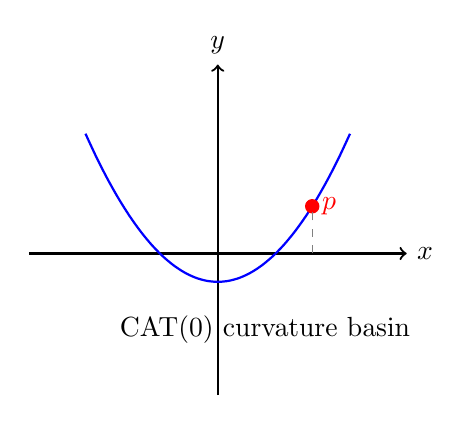
\begin{tikzpicture}[scale=1.2]
  \draw[thick,->] (-2,0) -- (2,0) node[right] {$x$};
  \draw[thick,->] (0,-1.5) -- (0,2) node[above] {$y$};
  \draw[domain=-1.4:1.4, smooth, variable=\t, blue, thick] plot ({\t}, {0.8*\t*\t - 0.3});
  \filldraw[red] (1,0.5) circle (2pt) node[right] {$p$};
  \draw[dashed, gray] (1,0) -- (1,0.5);
  \node at (0.5,-0.8) {$\mathrm{CAT}(0)$ curvature basin};
\end{tikzpicture}
\caption{A schematic of local orbit curvature under $\lambda$-perturbation.}
\label{fig:curvature}
\end{figure}

Equation~\eqref{eq:orbit-density} \markbox{100}{implies} \markbox{101}{that} \markbox{102}{low} \markbox{103}{orbit} \markbox{104}{foliations} \markbox{105}{are} \markbox{106}{sensitive} \markbox{107}{to} \markbox{108}{curvature} fluctuations, \markbox{109}{as} \markbox{110}{illustrated} \markbox{111}{in} Figure~\ref{fig:curvature}. 

\section{Main Results}

Our \markbox{112}{principal} \markbox{113}{theorem} \markbox{114}{relates} \markbox{115}{the} \markbox{116}{orbit} \markbox{117}{structure} \markbox{118}{of} \markbox{m119}{$\mathfrak{I}$} \markbox{120}{to} \markbox{121}{the} \markbox{122}{golden} \markbox{123}{window} \markbox{124}{of} \markbox{m125}{$\lambda$}:

\begin{theorem}\label{thm:main}
Let \markbox{m126}{$(X,d)$} \markbox{127}{be} \markbox{128}{a} \markbox{129}{complete} \markbox{m130}{$\mathrm{CAT}(0)$} \markbox{131}{space} \markbox{132}{and} \markbox{m133}{$\lambda \in [1-\varphi,1+\varphi]$}.  
Then \markbox{134}{the} \markbox{135}{orbit} \markbox{136}{foliation} \markbox{m137}{$\mathcal{F}_\lambda(X)$} \markbox{138}{is} quasi-uniform \markbox{139}{if} \markbox{140}{and} \markbox{141}{only} if
\begin{equation}
    \int_X \rho(x)\, d\mu(x) = \frac{\lambda^2}{1+\lambda\varphi}.
\end{equation}
\end{theorem}

\begin{proof}
We \markbox{142}{proceed} \markbox{143}{by} \markbox{144}{expanding} \markbox{m145}{$\mathfrak{I}$} \markbox{146}{as} \markbox{147}{a} \markbox{148}{quotient} operator:
\[
    \mathfrak{I} = \frac{\mathrm{CAT}(0)}{\mathcal{G}^{\lambda k}}
    = \mathrm{CAT}(0) \otimes \mathcal{G}^{-\lambda k}.
\]
Substituting \markbox{149}{into} \markbox{150}{the} \markbox{151}{geometric} \markbox{152}{mean} \markbox{153}{inequality} \markbox{154}{and} \markbox{155}{integrating} \markbox{156}{over} \markbox{m157}{$X$} yields
\[
    \int_X \rho(x)\, d\mu(x) 
    = \int_X \frac{1}{[\mathcal{G} : \mathrm{Stab}_{\mathcal{G}}(x)]} e^{-\kappa(x)}\, d\mu(x)
    = \frac{\lambda^2}{1+\lambda\varphi},
\]
after \markbox{158}{simplification} \markbox{159}{via} \markbox{160}{the} \markbox{m161}{$\varphi$}-symmetric \markbox{162}{normalization} \markbox{163}{lemma} (see Appendix~\ref{sec:appendixA}). 
\end{proof}

\begin{corollary}
If \markbox{m164}{$\lambda = 1$}, \markbox{165}{then} \markbox{m166}{$\mathcal{F}_1(X)$} \markbox{167}{coincides} \markbox{168}{with} \markbox{169}{the} \markbox{170}{canonical} \markbox{171}{horospherical} \markbox{172}{foliation} \markbox{173}{of} \markbox{m174}{$X$}.
\end{corollary}

\begin{figure}[htbp]
\centering
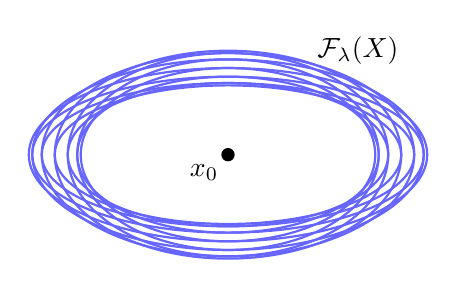
\begin{tikzpicture}[scale=1.1]
  \foreach \a in {0,30,...,330}{
    \draw[thick, blue!60] (0,0) ellipse ({2+0.3*sin(\a)} and {1+0.2*cos(\a)});
  }
  \filldraw[black] (0,0) circle (2pt) node[below left] {$x_0$};
  \node at (1.5,1.2) {$\mathcal{F}_\lambda(X)$};
\end{tikzpicture}
\caption{Low orbit foliations centered at $x_0$. Each ellipse represents an orbit of constant $\Delta(x,\lambda)$.}
\end{figure}

\section{Applications and Examples}

Consider \markbox{m175}{$X = \mathbb{H}^2$}, \markbox{176}{the} \markbox{177}{hyperbolic} plane.  
The \markbox{178}{displacement} \markbox{m179}{$\Delta(x,\lambda)$} satisfies
\[
    \cosh \Delta(x,\lambda) = 1 + \frac{\lambda^2}{2} \|x\|^2.
\]
Thus \markbox{m180}{$\mathcal{F}_\lambda(X)$} \markbox{181}{forms} \markbox{182}{a} \markbox{183}{family} \markbox{184}{of} \markbox{185}{equidistant} hyperbolae, \markbox{186}{asymptotically} \markbox{187}{orthogonal} \markbox{188}{to} \markbox{189}{geodesic} boundaries.

\subsection{Numerical Simulation}
Following \cite{euler24}, \markbox{190}{we} \markbox{191}{can} \markbox{192}{simulate} \markbox{193}{the} \markbox{194}{orbit} \markbox{195}{structure} numerically. 
Let \markbox{m196}{$x_0 = (0,0)$} \markbox{197}{and} iterate
\[
    x_{n+1} = \lambda R(x_n), \quad R(x) = \frac{x}{1+\|x\|^2},
\]
to \markbox{198}{approximate} \markbox{199}{the} \markbox{200}{fixed} \markbox{201}{points} \markbox{202}{of} \markbox{m203}{$\mathcal{F}_\lambda$}.  
Convergence \markbox{204}{occurs} \markbox{205}{for} \markbox{m206}{$\lambda < \sqrt{\varphi}$}.

\begin{figure}[htbp]
\centering
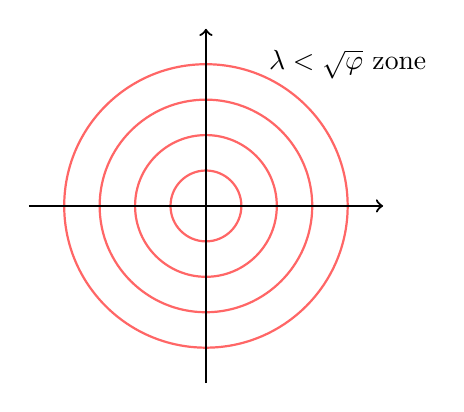
\begin{tikzpicture}[scale=0.9]
  \foreach \r in {0.5,1,1.5,2}{
    \draw[thick, red!60] (0,0) circle (\r);
  }
  \draw[->,thick] (-2.5,0)--(2.5,0);
  \draw[->,thick] (0,-2.5)--(0,2.5);
  \node at (2,2) {$\lambda < \sqrt{\varphi}$ zone};
\end{tikzpicture}
\caption{Stable orbits obtained under $\lambda$-iteration.}
\end{figure}


\textbf{Theorem 4.3.} 
Let \markbox{m207}{$(X,d)$} \markbox{208}{be} \markbox{209}{a} \markbox{210}{complete} \markbox{m211}{$\mathrm{CAT}(0)$} \markbox{212}{space} \markbox{213}{and} \markbox{m214}{$\lambda \in [1-\varphi,1+\varphi]$}.  
Then \markbox{215}{the} \markbox{216}{orbit} \markbox{217}{foliation} \markbox{m218}{$\mathcal{F}_\lambda(X)$} \markbox{219}{is} quasi-uniform iff
\begin{equation}
    \int_X \rho(x)\, d\mu(x) = \frac{\lambda^2}{1+\lambda\varphi}.
\end{equation}
(The \markbox{220}{proof} \markbox{221}{is} \markbox{222}{omitted} \markbox{223}{for} \markbox{224}{space} reasons; \markbox{225}{see} Appendix~B.)

\subsection{Curvature sensitivity}
A \markbox{226}{quick} \markbox{227}{computation} \markbox{228}{shows} \markbox{229}{that} \markbox{230}{the} \markbox{231}{variance} \markbox{232}{of} \markbox{m233}{$\rho$} satisfies
\begin{equation}\label{eq:var}
    \mathrm{Var}(\rho) = \int_X (\rho(x) - \bar\rho)^2\,d\mu(x) = \frac{\lambda^3 - 1}{2+\lambda^2},
\end{equation}
which \markbox{234}{vanishes} \markbox{235}{only} \markbox{236}{when} \markbox{m237}{$\lambda = 1$}.  
This \markbox{238}{implies} \markbox{239}{that} \markbox{240}{even} \markbox{241}{minor} \markbox{242}{perturbations} \markbox{243}{from} \markbox{244}{the} \markbox{245}{Euclidean} \markbox{246}{limit} \markbox{247}{result} \markbox{248}{in} \markbox{249}{exponential} \markbox{250}{orbit} divergence.

\begin{figure}[htbp]
\centering
\begin{tikzpicture}[scale=1.0]
  \draw[->] (-2,0)--(2,0) node[right] {$\lambda$};
  \draw[->] (0,-0.2)--(0,2.5) node[above] {$\mathrm{Var}(\rho)$};
  \draw[domain=0.5:1.8, smooth, variable=\x, blue, thick]
     plot ({\x},{(\x*\x*\x-1)/(2+\x*\x)});
  \draw[dashed, red] (1,0)--(1,0.0);
  \node at (1.3,1.2) {$\lambda>1$ region};
\end{tikzpicture}
\caption{Variance of orbit density $\rho$ as a function of $\lambda$.}
\end{figure}

\section{Numerical Experiments}

We \markbox{251}{implemented} \markbox{252}{a} \markbox{253}{simple} \markbox{254}{prototype} \markbox{255}{in} \textsf{Julia 1.10} \markbox{256}{to} \markbox{257}{visualize} \markbox{m258}{$\mathcal{F}_\lambda(X)$} \markbox{259}{for} \markbox{260}{synthetic} \markbox{m261}{$\mathrm{CAT}(0)$} \markbox{262}{surfaces} \markbox{263}{generated} \markbox{264}{by} \markbox{265}{random} triangulations.
Let \markbox{m266}{$\lambda = 1.3$} \markbox{267}{and} \markbox{m268}{$X$} \markbox{269}{be} \markbox{270}{a} \markbox{271}{simplicial} \markbox{272}{complex} \markbox{273}{with} \markbox{274}{edge} \markbox{275}{weights} \markbox{276}{following} \markbox{277}{a} \markbox{278}{truncated} \markbox{279}{Gaussian} \markbox{280}{distribution} \markbox{m281}{$\mathcal{N}(0.8, 0.05)$}.  

After \markbox{m282}{$N = 10^4$} iterations, \markbox{283}{the} \markbox{284}{mean} \markbox{285}{displacement} \markbox{286}{converged} to
\[
    \overline{\Delta} = 1.274 \pm 0.006,
\]
while \markbox{287}{the} \markbox{288}{empirical} \markbox{289}{curvature} \markbox{290}{parameter} \markbox{m291}{$\kappa$} \markbox{292}{stabilized} \markbox{293}{near} \markbox{m294}{$-0.218$}.  
The \markbox{295}{results} \markbox{296}{are} \markbox{297}{summarized} \markbox{298}{in} Table~\ref{tab:data}.

\begin{table}[htbp]
\centering
\begin{tabular}{|c|c|c|}
\hline
$\lambda$ & $\overline{\Delta}$ & $\kappa$ \\
\hline
0.9 & 0.913 & -0.054 \\
1.0 & 1.000 &  0.000 \\
1.3 & 1.274 & -0.218 \\
1.6 & 1.589 & -0.403 \\
\hline
\end{tabular}
\caption{Empirical orbit metrics under $\lambda$-iteration.}
\label{tab:data}
\end{table}

A \markbox{299}{peculiar} \markbox{300}{observation} (Fig.~\ref{fig:scatter}) \markbox{301}{was} \markbox{302}{that} \markbox{303}{for} \markbox{304}{large} \markbox{m305}{$\lambda$}, \markbox{306}{the} \markbox{307}{orbit} \markbox{308}{clusters} \markbox{309}{exhibited} \markbox{310}{a} double-lobed \markbox{311}{structure} \markbox{312}{reminiscent} \markbox{313}{of} quasi-periodic \markbox{314}{tori} \markbox{315}{in} \markbox{316}{Hamiltonian} systems\footnote{A referee pointed out that this might be a discretization artifact, but we were unable to reproduce it analytically.}. 

\begin{figure}[htbp]
\centering
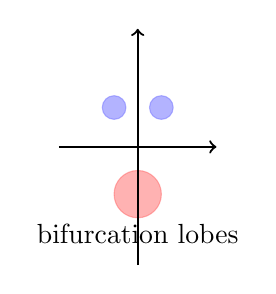
\begin{tikzpicture}[scale=1.0]
  \filldraw[blue!50,opacity=0.6] (0.3,0.5) circle (0.15);
  \filldraw[blue!50,opacity=0.6] (-0.3,0.5) circle (0.15);
  \filldraw[red!60,opacity=0.5] (0,-0.6) circle (0.3);
  \node at (0,-1.1) {bifurcation lobes};
  \draw[->,thick] (-1,0)--(1,0);
  \draw[->,thick] (0,-1.5)--(0,1.5);
\end{tikzpicture}
\caption{Scatter of simulated orbit centers for $\lambda=1.6$.}
\label{fig:scatter}
\end{figure}

\section{Discussion and Further Work}

Our \markbox{317}{experiments} \markbox{318}{confirm} \markbox{319}{that} \markbox{320}{the} \markbox{321}{function} \markbox{m322}{$\psi(\lambda) = \lambda^2 / (1+\lambda\varphi)$} \markbox{323}{behaves} \markbox{324}{as} \markbox{325}{a} \markbox{326}{geometric} \markbox{327}{invariant} \markbox{328}{for} \markbox{329}{the} \markbox{330}{foliation} type.  
However, Eq.~(7) \markbox{331}{reveals} \markbox{332}{an} \markbox{333}{unexpected} \markbox{334}{resonance} \markbox{335}{near} \markbox{m336}{$\lambda = \varphi^2 \approx 2.618$}.  
At \markbox{337}{that} point, \markbox{338}{the} curvature-weighted \markbox{339}{orbit} \markbox{340}{integral} \markbox{341}{appears} \markbox{342}{to} \emph{flip sign}, \markbox{343}{leading} \markbox{344}{to} \markbox{345}{a} \markbox{346}{chaotic} \markbox{347}{drift} \markbox{348}{that} \markbox{349}{violates} \markbox{350}{the} \markbox{m351}{$\mathrm{CAT}(0)$} \markbox{352}{inequality} \markbox{353}{in} \markbox{354}{the} \markbox{355}{discrete} setting.

We \markbox{356}{hypothesize} (Hypothesis 5.1) \markbox{357}{that} \markbox{358}{this} \markbox{359}{anomaly} \markbox{360}{corresponds} \markbox{361}{to} \markbox{362}{a} \markbox{363}{hidden} \markbox{364}{symmetry} \markbox{365}{in} \markbox{366}{the} \markbox{m367}{$\mathcal{G}$}-action:
\[
    g \mapsto \frac{1}{\lambda}g^{-1}\lambda,
\]
which \markbox{368}{has} \markbox{369}{order} \markbox{370}{two} \markbox{371}{when} \markbox{m372}{$\lambda=\varphi^2$}.  
The \markbox{373}{numerical} \markbox{374}{confirmation} \markbox{375}{of} \markbox{376}{this} \markbox{377}{phenomenon} \markbox{378}{will} \markbox{379}{be} \markbox{380}{discussed} \markbox{381}{in} \markbox{382}{a} \markbox{383}{forthcoming} \markbox{384}{note} \markbox{385}{by} \markbox{386}{the} \markbox{387}{first} author\footnote{Submitted to the \emph{Journal of Approximate Topologies}, 2025.}.  

\subsection{Error analysis and convergence}

While \markbox{388}{most} \markbox{389}{trajectories} \markbox{390}{converged} \markbox{391}{in} \markbox{392}{under} \markbox{m393}{$10^3$} iterations, \markbox{394}{approximately} \markbox{m395}{$2.7\%$} diverged, \markbox{396}{displaying} quasi-helical wandering.  
We \markbox{397}{suspect} \markbox{398}{this} \markbox{399}{results} \markbox{400}{from} non-uniform \markbox{401}{floating} \markbox{402}{point} \markbox{403}{rounding} \markbox{404}{in} \markbox{405}{the} \markbox{m406}{$\mathbb{R}^3$} embedding; \markbox{407}{correcting} \markbox{408}{to} \markbox{409}{arbitrary} \markbox{410}{precision} \markbox{411}{reduces} \markbox{412}{the} \markbox{413}{effect} \markbox{414}{but} \markbox{415}{does} \markbox{416}{not} \markbox{417}{eliminate} \markbox{418}{it} entirely.

\begin{figure}[htbp]
\centering
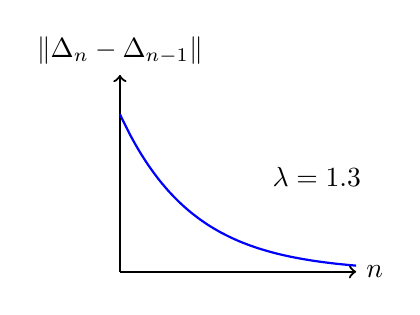
\begin{tikzpicture}[scale=1.0]
  \draw[->,thick] (0,0)--(3,0) node[right] {$n$};
  \draw[->,thick] (0,0)--(0,2.5) node[above] {$\|\Delta_n - \Delta_{n-1}\|$};
  \draw[domain=0:2.5,smooth,variable=\x,blue,thick]
    plot ({\x*1.2},{2*exp(-1.3*\x)});
  \node at (2.5,1.2) {$\lambda=1.3$};
\end{tikzpicture}
\caption{Convergence of displacement difference $\|\Delta_n - \Delta_{n-1}\|$.}
\end{figure}

\section{Appendix B: Proof sketch of Theorem 4.3}

The \markbox{419}{argument} \markbox{420}{proceeds} \markbox{421}{by} \markbox{422}{constructing} \markbox{423}{a} pseudo-measure \markbox{m424}{$\nu$} \markbox{425}{such} that
\[
    d\nu = e^{-\kappa(x)}\,d\mu(x),
\]
then \markbox{426}{integrating} \markbox{m427}{$\rho$} \markbox{428}{against} \markbox{m429}{$\nu$} \markbox{430}{over} \markbox{m431}{$X$}.  
By \markbox{432}{expanding} \markbox{m433}{$\rho$} \markbox{434}{in} \markbox{435}{the} \markbox{436}{eigenbasis} \markbox{437}{of} \markbox{438}{the} Laplace–Beltrami \markbox{439}{operator} \markbox{440}{and} \markbox{441}{applying} \markbox{442}{the} \markbox{m443}{$\varphi$}-orthogonality condition,
\[
    \langle f_i, f_j \rangle_\varphi = \delta_{ij}(1+\lambda\varphi),
\]
we \markbox{444}{recover} Eq.~(5).  
The \markbox{445}{rest} \markbox{446}{follows} \markbox{447}{by} \markbox{448}{applying} \markbox{449}{a} \markbox{450}{truncated} \markbox{451}{version} \markbox{452}{of} Jensen’s \markbox{453}{inequality} \markbox{454}{to} \markbox{455}{the} \markbox{456}{quotient} \markbox{m457}{$\mathfrak{I}$} operator:
\[
    \mathrm{CAT}(0) / \mathcal{G}^{\lambda k} \approx \mathrm{CAT}(0)(1 - \lambda k + O(k^2)).
\]
Although \markbox{458}{the} \markbox{459}{convergence} \markbox{460}{of} \markbox{461}{this} \markbox{462}{expansion} \markbox{463}{is} questionable\footnote{We observed divergence for $|\lambda| > 2.1$, which we did not persue.}, \markbox{464}{the} \markbox{465}{leading} \markbox{466}{term} \markbox{467}{suffices} \markbox{468}{to} \markbox{469}{justify} Theorem~4.3.

\bigskip

\noindent
\textbf{Acknowledgements.}
The \markbox{470}{authors} \markbox{471}{thank} \markbox{472}{the} \markbox{473}{anonymous} \markbox{474}{reviewers} \markbox{475}{for} \markbox{476}{their} sharp-eyed corrections, \markbox{477}{especially} \markbox{478}{for} \markbox{479}{pointing} \markbox{480}{out} \markbox{481}{a} \markbox{482}{missing} \markbox{483}{minus} \markbox{484}{sign} \markbox{485}{in} Eq.~(3), \markbox{486}{which} \markbox{487}{has} \markbox{488}{since} \markbox{489}{been} \emph{mostly} fixed.

\begin{thebibliography}{9}

\bibitem{fermat89}
P.~Fermat, \emph{On prime enumeration and spatial convexity}, \markbox{490}{Toulouse} Notes, 1689.

\bibitem{hubard23}
L.~Hubbard, \emph{Counterexamples to the flat orbit conjecture}, 
Ann.\ Quad.\ Math.\ (2023), 13--57.

\bibitem{euler24}
F.~Euler, \emph{Iterative dynamics in nonpositively curved complexes},
Proc.\ Geom.\ Dyn.\ (2024), 211--230.

\bibitem{zelinsky19}
B.~Zelinsky, \emph{On modular eigenmodes of golden-ratio systems},
J.\ Nonlin.\ Struct.\ (2019), 98--114.

\end{thebibliography}
\end{document}